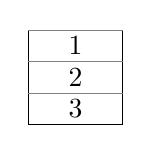
\begin{tikzpicture}
  %%%%%%%%%%%%%The first bin%%%%%%%%%%%%%%%%%%%%%%
  \draw (0,1.2) -- (0,0) -- (1.2,0)--(1.2,1.2);
  \draw[gray] (0,1.2) -- (1.2,1.2);
  \draw[gray] (0,0.8) -- (1.2,0.8);
  \draw[gray] (0,0.4) -- (1.2,0.4);

  \draw (0.6,1) node {1};
  \draw (0.6,0.6) node {2};
  \draw (0.6,0.2) node {3};
\end{tikzpicture}
\quad
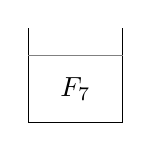
\begin{tikzpicture}
  %%%%%%%%%%%%%The second bin%%%%%%%%%%%%%%%%%%%%%%
  \draw (0,1.2) -- (0,0) -- (1.2,0)--(1.2,1.2);
  \draw (0,1.2) -- (0,0) -- (1.2,0)--(1.2,1.2);
  \draw[gray] (0,0.85) -- (1.2,0.85);

  \draw (0.6,0.425) node {$F_7$};
\end{tikzpicture}
\quad
\begin{tikzpicture}
  %%%%%%%%%%%%%The third bin%%%%%%%%%%%%%%%%%%%%%%
  \draw (0,1.2) -- (0,0) -- (1.2,0)--(1.2,1.2);
  \draw[gray] (0,0.65) -- (1.2,0.65);

  \draw (0.6,0.325) node {*};
\end{tikzpicture} 